%%%%%%%%%%%%%%%%%%%%%%%%%%%%%%%%%%%%%%%%%%%%%%%%%%%%%%%%%%%%%%%%
%
%  Template for homework of Introduction to Machine Learning.
%
%  Fill in your name, lecture number, lecture date and body
%  of homework as indicated below.
%
%%%%%%%%%%%%%%%%%%%%%%%%%%%%%%%%%%%%%%%%%%%%%%%%%%%%%%%%%%%%%%%%


\documentclass[11pt,letter,notitlepage]{article}
%Mise en page
\usepackage[left=2cm, right=2cm, lines=45, top=0.8in, bottom=0.7in]{geometry}
\usepackage{fancyhdr}
\usepackage{fancybox}
\usepackage{graphicx}
\usepackage{pdfpages} 
\usepackage{enumitem}
\usepackage{algorithm}
\usepackage{algorithmic}
\renewcommand{\headrulewidth}{1.5pt}
\renewcommand{\footrulewidth}{1.5pt}
\newcommand\Loadedframemethod{TikZ}
\usepackage[framemethod=\Loadedframemethod]{mdframed}

\usepackage{amssymb,amsmath}
\usepackage{amsthm}
\usepackage{thmtools}
\newtheorem{lemma}{Lemma}

\setlength{\topmargin}{0pt}
\setlength{\textheight}{9in}
\setlength{\headheight}{0pt}

\setlength{\oddsidemargin}{0.25in}
\setlength{\textwidth}{6in}

\usepackage{graphicx} % more modern
\usepackage{subfigure}
\usepackage{threeparttable}
\usepackage{ctex}

%%%%%%%%%%%%%%%%%%%%%%%%
%%%%%% Define math operator %%%%%
%%%%%%%%%%%%%%%%%%%%%%%%
\DeclareMathOperator*{\argmin}{\bf argmin}
\DeclareMathOperator*{\relint}{\bf relint\,}
\DeclareMathOperator*{\dom}{\bf dom\,}
\DeclareMathOperator*{\intp}{\bf int\,}
%%%%%%%%%%%%%%%%%%%%%%%


\setlength{\topmargin}{0pt}
\setlength{\textheight}{9in}
\setlength{\headheight}{0pt}

\setlength{\oddsidemargin}{0.25in}
\setlength{\textwidth}{6in}
\pagestyle{fancy}
%%%%%%%%%%%%%%%%%%%%%%%%
%% Define the Exercise environment %%
%%%%%%%%%%%%%%%%%%%%%%%%
\mdtheorem[
topline=false,
rightline=false,
leftline=false,
bottomline=false,
leftmargin=-10,
rightmargin=-10
]{exercise}{\textbf{Exercise}}
%%%%%%%%%%%%%%%%%%%%%%%
%% End of the Exercise environment %%
%%%%%%%%%%%%%%%%%%%%%%%


%%%%%%%%%%%%%%%%%%%%%%%%
%% Define the Problem environment %%
%%%%%%%%%%%%%%%%%%%%%%%%
\mdtheorem[
topline=false,
rightline=false,
leftline=false,
bottomline=false,
leftmargin=-10,
rightmargin=-10
]{problem}{\textbf{Problem}}
%%%%%%%%%%%%%%%%%%%%%%%
%% End of the Exercise environment %%
%%%%%%%%%%%%%%%%%%%%%%%

%%%%%%%%%%%%%%%%%%%%%%%
%% Define the Solution Environment %%
%%%%%%%%%%%%%%%%%%%%%%%
\declaretheoremstyle
[
spaceabove=0pt, 
spacebelow=0pt, 
headfont=\normalfont\bfseries,
notefont=\mdseries, 
notebraces={(}{)}, 
headpunct={:\quad}, 
headindent={},
postheadspace={ }, 
postheadspace=4pt, 
bodyfont=\normalfont, 
qed=$\blacksquare$,
preheadhook={\begin{mdframed}[style=myframedstyle]},
	postfoothook=\end{mdframed},
]{mystyle}

\declaretheorem[style=mystyle,title=Solution,numbered=no]{solution}
\mdfdefinestyle{myframedstyle}{%
	topline=false,
	rightline=false,
	leftline=false,
	bottomline=false,
	skipabove=-6ex,
	leftmargin=-10,
	rightmargin=-10}
%%%%%%%%%%%%%%%%%%%%%%%
%% End of the Solution environment %%
%%%%%%%%%%%%%%%%%%%%%%%

%% Homework info.
\newcommand{\posted}{\text{Nov. 20, 2019}}       			%%% FILL IN POST DATE HERE
\newcommand{\due}{\text{Nov. 27, 2019}} 			%%% FILL IN Due DATE HERE
\newcommand{\hwno}{\text{5}} 		           			%%% FILL IN LECTURE NUMBER HERE


%%%%%%%%%%%%%%%%%%%%
%% Put your information here %%
%%%%%%%%%%%%%%%%%%%
\newcommand{\name}{\text{Jiahuan Yu}}  	          			%%% FILL IN YOUR NAME HERE
\newcommand{\id}{\text{PB17121687}}		       			%%% FILL IN YOUR ID HERE
%%%%%%%%%%%%%%%%%%%%
%% End of the student's info %%
%%%%%%%%%%%%%%%%%%%


\newcommand{\proj}[2]{\textbf{P}_{#2} (#1)}
\newcommand{\lspan}[1]{\textbf{span}  (#1)  }
\newcommand{\rank}[1]{ \textbf{rank}  (#1)  }
\newcommand{\RNum}[1]{\uppercase\expandafter{\romannumeral #1\relax}}


\lhead{
	\textbf{\name}
}
\rhead{
	\textbf{\id}
}
\chead{\textbf{
		Homework \hwno
}}


\begin{document}
\vspace*{-4\baselineskip}
\thispagestyle{empty}


\begin{center}
	{\bf\large Introduction to Machine Learning}\\
	{Fall 2019}\\
	University of Science and Technology of China
\end{center}

\noindent
Lecturer: Jie Wang  			 %%% FILL IN LECTURER HERE
\hfill
Homework \hwno
\\
Posted: \posted
\hfill
Due: \due
\\
Name: \name
\hfill
ID: \id
\hfill

\noindent
\rule{\textwidth}{2pt}

\medskip





%%%%%%%%%%%%%%%%%%%%%%%%%%%%%%%%%%%%%%%%%%%%%%%%%%%%%%%%%%%%%%%%
%% BODY OF HOMEWORK GOES HERE
%%%%%%%%%%%%%%%%%%%%%%%%%%%%%%%%%%%%%%%%%%%%%%%%%%%%%%%%%%%%%%%%

\textbf{Notice, }to get the full credits, please show your solutions step by step.

\begin{exercise}[Decision Tree  \textnormal{10pts}]
	Please build a decision tree based on the information gain to classify the following dataset (you need to show the calculation steps in detail).
\end{exercise}
\begin{table}[h]
	\centering
	\begin{tabular}{|c|c|c|c|c|c|}
		\hline
		Sample & $A_1$ & $A_2$ & $A_3$ & Response \\
		\hline
		$x_1$  & 1     & 0     & 0     & 0        \\
		$x_2$  & 1     & 0     & 1     & 0        \\
		$x_3$  & 0     & 1     & 0     & 0        \\
		$x_4$  & 1     & 1     & 1     & 1        \\
		$x_5$  & 1     & 1     & 0     & 1        \\
		\hline
	\end{tabular}
	\caption{Dataset} \label{tab:sample}
	{\raggedright The dataset consists of five samples $x_1,x_2,x_3,x_4,x_5$. For each sample, we can observe the features $A_1,A_2,A_3$ and the corresponding response. \par}
\end{table}
\begin{solution}
	$$S_0=\{x_1,x_2,x_3,x_4,x_5\}$$ \\
	对 $S_0$ 进行计算:
	$$\begin{aligned}
			{\rm Entropy}(S_0)
			 & = -\cfrac{3}{5}\log_2\cfrac{3}{5}-\cfrac{2}{5}\log_2\cfrac{2}{5}=0.97                    \\
			{\rm Gain}(S_0,A_1)
			 & = {\rm Entropy}(S_0)-\sum_{A_1\in\{0,1\}}\cfrac{|S_{A_1}|}{|S_0|}{\rm Entropy}(S_{A_1})  \\
			 & =0.97
			-\cfrac{1}{5}\times0
			-\cfrac{4}{5}\times\left(-\cfrac{2}{4}\log_2\cfrac{2}{4}-\cfrac{2}{4}\log_2\cfrac{2}{4}\right)
			=0.17                                                                                       \\
			{\rm Gain}(S_0,A_2)
			 & = {\rm Entropy}(S_0)-\sum_{A_2\in\{0,1\}}\cfrac{|S_{A_2}|}{|S_0|}{\rm Entropy}(S_{A_2})  \\
			 & =0.97
			-\cfrac{2}{5}\times0
			-\cfrac{3}{5}\times\left(-\cfrac{1}{3}\log_2\cfrac{1}{3}-\cfrac{2}{3}\log_2\cfrac{2}{3}\right)
			=0.42                                                                                       \\
			{\rm Gain}(S_0,A_3)
			 & = {\rm Entropy}(S_0) -\sum_{A_3\in\{0,1\}}\cfrac{|S_{A_3}|}{|S_0|}{\rm Entropy}(S_{A_3}) \\
			 & =0.97
			-\cfrac{3}{5}\times\left(-\cfrac{2}{3}\log_2\cfrac{2}{3}-\cfrac{1}{3}\log_2\cfrac{1}{3}\right)
			-\cfrac{2}{5}\times\left(-\cfrac{1}{2}\log_2\cfrac{1}{2}-\cfrac{1}{2}\log_2\cfrac{1}{2}\right)
			=0.02
		\end{aligned}$$
	所以选 $A_2$ 进行划分:
	$$\begin{aligned}
			S_1 & =\{x_1,x_2\}     \\
			S_2 & =\{x_3,x_4,x_5\}
		\end{aligned}$$
	$S_1$ 中的全部样本 $Response=0$, 所以 $S_1$ 对应的 $Response=0$. \\
	对 $S_2$ 进行计算:
	$$\begin{aligned}
			{\rm Entropy}(S_2)
			 & = -\cfrac{1}{3}\log_2\cfrac{1}{3}-\cfrac{2}{3}\log_2\cfrac{2}{3}=0.92                   \\
			{\rm Gain}(S_2,A_1)
			 & = {\rm Entropy}(S_2)-\sum_{A_1\in\{0,1\}}\cfrac{|S_{A_1}|}{|S_2|}{\rm Entropy}(S_{A_1}) \\
			 & =0.92
			-\cfrac{1}{3}\times0
			-\cfrac{2}{3}\times0
			=0.92                                                                                      \\
			{\rm Gain}(S_2,A_3)
			 & = {\rm Entropy}(S_2)-\sum_{A_3\in\{0,1\}}\cfrac{|S_{A_3}|}{|S_2|}{\rm Entropy}(S_{A_3}) \\
			 & =0.92
			-\cfrac{2}{3}\times\left(-\cfrac{1}{2}\log_2\cfrac{1}{2}-\cfrac{1}{2}\log_2\cfrac{1}{2}\right)
			-\cfrac{1}{3}\times0
			=0.25
		\end{aligned}$$
	所以选 $A_1$ 进行划分:
	$$\begin{aligned}
			S_3 & =\{x_3\}     \\
			S_4 & =\{x_4,x_5\}
		\end{aligned}$$
	$S_3$ 中的全部样本 $Response=0$, 所以 $S_1$ 对应的 $Response=0$. \\
	$S_4$ 中的全部样本 $Response=1$, 所以 $S_1$ 对应的 $Response=1$. \\
	最后生成的决策树为: \\
	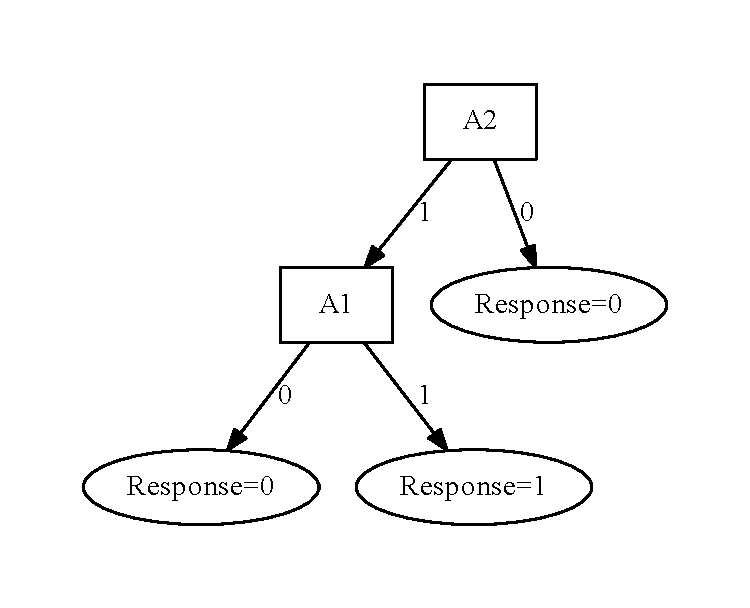
\includegraphics{solution1_tree.pdf}

\end{solution}
\newpage

\begin{exercise}[Softmax and Cross Entropy  \textnormal{30pts}]
	The softmax function $f:\mathbb{R}^n\rightarrow\mathbb{R}^n$ is defined by:
	$$f_i(x)=\frac{\exp(x_i)}{\sum_{k=1}^{n}\exp(x_k)}, i=1,\ldots,n,$$
	where $x_i$ is the $i^{th}$ component of $x\in\mathbb{R}^n$. The function  $f(x)=(f_1(x),f_2(x),\ldots,f_n(x))^{\top}$ converts each input $x$ into a probability (stochastic) vector in which all entries are nonnegative and add up to one.
	\begin{itemize}
		\item[1.] Please find the gradient and Jacobian of $f(x)$, i.e., $\nabla f(x)$ and $Df(x)$.

		\item[2.] Show that $f(x)=f(x-c)$, where $c=\max\{x_1,x_2,...,x_n\}$. When could we need this transformation?

		\item[3.] Please find the gradient of cross entropy function:
		      $$g(x)=-\sum_{i=1}^{n}H_i\log(f_i(x)),$$
		      where $H\in\mathbb{R}^n$ is a one-hot vector.
	\end{itemize}
\end{exercise}

\begin{solution}
	\begin{enumerate}
		\item $$\cfrac{\partial f_i}{\partial x_j} = \begin{cases}
				      -\cfrac{\exp(x_i)\exp(x_j)}{\left( \sum_{k=1}^{n}{\exp(x_k)} \right)^2}
				      = -f_i f_j
				       & , i \neq j \\
				      \cfrac{\exp(x_i)\sum_{k=1}^{n}{\exp(x_k)} - (\exp(x_i))^2}{\left( \sum_{k=1}^{n}{\exp(x_k)} \right)^2}
				      =f_i - f_i^2
				       & , i = j
			      \end{cases}$$
		      所以
		      $$ \nabla f(x)
			      = \begin{pmatrix}
				      \cfrac{\partial f_1}{\partial x_1} & \cfrac{\partial f_2}{\partial x_1} & \cdots & \cfrac{\partial f_n}{\partial x_1} \\
				      \cfrac{\partial f_1}{\partial x_2} & \cfrac{\partial f_2}{\partial x_2} & \cdots & \cfrac{\partial f_n}{\partial x_2} \\
				      \vdots                             & \vdots                             & \ddots & \vdots                             \\
				      \cfrac{\partial f_1}{\partial x_n} & \cfrac{\partial f_2}{\partial x_n} & \cdots & \cfrac{\partial f_n}{\partial x_n}
			      \end{pmatrix}= \begin{pmatrix}
				      f_1-f_1^2 & -f_2 f_1  & \cdots & -f_n f_1  \\
				      -f_1 f_2  & f_2-f_2^2 & \cdots & -f_n f_2  \\
				      \vdots    & \vdots    & \ddots & \vdots    \\
				      -f_1 f_n  & -f_2 f_n  & \cdots & f_n-f_n^2
			      \end{pmatrix}$$
		      $$D f= (\nabla f)^\top=\begin{pmatrix}
				      f_1-f_1^2 & -f_1 f_2  & \cdots & -f_1 f_n  \\
				      -f_2 f_1  & f_2-f_2^2 & \cdots & -f_2 f_n  \\
				      \vdots    & \vdots    & \ddots & \vdots    \\
				      -f_n f_1  & -f_n f_2  & \cdots & f_n-f_n^2
			      \end{pmatrix}$$
		\item $$f_i(x-c)=\cfrac{\exp(x_i-c)}{\sum_{k=1}^{n}{\exp(x_k-c)}}=\cfrac{\exp(x_i)}{\sum_{k=1}^{n}{\exp(x_k)}}=f_i(x)$$
		      所以 $f(x-c)=f(x)$

		      当 $x_i$ 较大时,$\exp(x_i)$ 的计算容易导致溢出,因此设 $c=\max\{x_i\}, i=1,2,\cdots,n$.

		      则 $x_i-c \leq0$, 可以保证计算不会溢出。
		\item  $$\begin{aligned}
				      \cfrac{\partial g(x)}{\partial x_j}
				       & = -\sum_{i=1}^{n}{H_i\cfrac{\partial \log(f_i(x))}{\partial x_j}}                  \\
				       & = -\sum_{i=1}^{n}{\cfrac{H_i}{f_i(x)} \cfrac{\partial f_i(x)}{\partial x_j}}       \\
				       & = -\cfrac{H_j}{f_j(x)}(f_j-f_j^2) - \sum_{i\neq j}{\cfrac{H_i}{f_i(x)} (-f_i f_j)} \\
				       & = H_j (f_j-1) + \sum_{i\neq j}{H_i f_j}                                            \\
				       & = f_j - H_j
			      \end{aligned}$$
		      所以
		      $$\nabla g(x)=f(x)-H$$
	\end{enumerate}
\end{solution}

\newpage


\begin{exercise}[Convolutional Neural Network \textnormal{40pts}]
	\begin{enumerate}
		\item The average pooling in convolutional neural network can be formulated as
		      $$f_1(x)= \frac{\sum_{i=1}^n x_i}{n},$$
		      where $x_i$ is the $i^{th}$ component of $x\in\mathbb{R}^n$. Please derive the gradient of $f_1(x)$.
		\item The max pooling in convolutional neural network can be formulated as
		      $$f_2(x)= \max\{x_1,\dots,x_n\},$$
		      where $x_i$ is the $i^{th}$ component of $x\in\mathbb{R}^n$.
		      \begin{enumerate}
			      \item Find the set containing all differentiable points of of $f_2$.
			      \item We call $d(x)$ is a subgradient at $x$ $f_2$ if
			            \begin{align*}
				            f_2(y) \geq f_2(x) + \langle d(x),y-x \rangle, \forall x,y .
			            \end{align*}
			            Find a subgradient $d(x)$ of $f_2$ at $x$.
		      \end{enumerate}
		\item Suppose that we have a convolutional neural network as shown in Table \ref{tab:cnn}.
		      \begin{enumerate}
			      \item The convolutinal layer parameters are denoted as ``conv$\langle$filter size$\rangle$-$\langle$number of filters$\rangle$".
			      \item  The fully connected layer parameters are denoted as ``FC$\langle$number of neurons$\rangle$".
			      \item The window size of pooling layers is $3$.
			      \item The stride of convolutinal layers is $1$.
			      \item The stride of pooling layers is $3$.
			      \item There is no padding in both convolutional and pooling layers.
			      \item For convenience, we assume that there is no activation function and bias.
		      \end{enumerate}

		      Suppose that the input is a $\mathbf{386\times 386}$ \textbf{RGB} image. Please derive the size of all feature maps and the number of parameters.
	\end{enumerate}


\end{exercise}

\begin{table}[h]
	\centering
	\begin{tabular}{|c|c|c|c|c|c|c|}
		\hline
		conv3-64 & max pool & conv3-256 & conv1-512 & max pool & FC-2048 & FC-1000 \\
		\hline
	\end{tabular}
	\caption{The architecture of convolutional neural network} \label{tab:cnn}
\end{table}
\begin{solution}
	\begin{enumerate}
		\item $\nabla f_1(x) = \left( \cfrac{1}{n}, \cdots, \cfrac{1}{n} \right)^\top$
		\item \begin{enumerate}
			      \item \begin{enumerate}
				            \item 当 $\exists x_i=x_j=\max\{x_1,\cdots,x_n\} ,i\neq j$ 时,设 $\varepsilon>0$,令
				                  $$\begin{aligned}
						                  x'  & = \left( x_1,\cdots,x_i+\varepsilon,\cdots,x_n \right)^\top \\
						                  x'' & = \left( x_1,\cdots,x_i-\varepsilon,\cdots,x_n \right)^\top
					                  \end{aligned}$$
				                  则
				                  $$\begin{aligned}
						                  f_2(x')  & = x_i+\varepsilon \\
						                  f_2(x'') & = x_j
					                  \end{aligned}$$
				                  所以
				                  $$\begin{aligned}
						                  \lim_{\varepsilon\to0} \cfrac{f_2(x')-f_2(x)}{\varepsilon}  & =1 \\
						                  \lim_{\varepsilon\to0} \cfrac{f_2(x'')-f_2(x)}{\varepsilon} & =0
					                  \end{aligned}$$
				                  可知 $f_2(x)$ 在 $x$ 处对 $x_i$ 的偏导数不存在。

				                  所以在这点 $f_2(x)$ 不可微。
				            \item 当 $\exists x_i=\max\{x_1,\cdots,x_n\}$ 使得 $\forall j\neq i, x_j <x_i$ 时,设
				                  $$0<\varepsilon<\cfrac{1}{2}\min\{x_i-x_1,\cdots,x_i-x_{i-1},x_i-x_{i+1},\cdots,x_i-x_n\}$$

				                  则对于 $\forall x'$, 若 $\|x'-x\|\leq\varepsilon$,就有 $f_2(x')=x_i'$

				                  所以在某一邻域中 $f_2(x)=x_i$, 所以在 $x$ 处可导。
			            \end{enumerate}
			            综上,可导点的集合为 $\{ x \mid \exists x_i,\text{s.t. }x_j < x_i, \forall j\neq i\}$
			      \item 设 $f_2(x)=x_i$, 则
			            $$d(x)=(\underbrace{0,\cdots,0}_{\text{i-1 个 0}},\underbrace{1}_{\text{第 i 个分量为 1}},\underbrace{0,\cdots,0}_{\text{n-i 个 0}})^\top$$
			            是一个 subgradient. 证明如下:
			            $$f_2(x)+\langle d(x),y-x \rangle=x_i+(y_i-x_i)=y_i \leq f_2(y)$$
		      \end{enumerate}
		\item 每层计算后的 feature maps 和所用的参数数量如下: \\
		      \begin{center}
			      \begin{tabular}{|c|c|c|}
				      \hline
				      \textbf{Layer} & \textbf{size of feature maps}                       & \textbf{number of parameters}  \\
				      \hline
				      conv3-64       & $64\times(386-3+1)^2=9437184$                       & $3\times3^2\times64=1728$      \\
				      \hline
				      max pool       & $64\times\left(\cfrac{384-3}{3}+1\right)^2=1048576$ & 0                              \\
				      \hline
				      conv3-256      & $256\times(128-3+1)^2=4064256$                      & $64\times3^2\times256=147456$  \\
				      \hline
				      conv1-512      & $512\times(126-1+1)^2=8128512$                      & $256\times1^2\times512=131072$ \\
				      \hline
				      max pool       & $512\times\left(\cfrac{126-3}{3}+1\right)^2=903168$ & 0                              \\
				      \hline
				      FC-2048        & 2048                                                & $2048\times903168=1849688064$  \\
				      \hline
				      FC-1000        & 1000                                                & $1000\times2048=2048000$       \\
				      \hline
			      \end{tabular}
		      \end{center}
	\end{enumerate}
\end{solution}

\newpage

\begin{exercise}[Matrix Calculus \textnormal{20pts}]

	\indent Let $L = f(h(Ax+b))$, where $A \in \mathbb{R}^{m \times n}$, $x \in \mathbb{R}^n$, $b \in \mathbb{R}^m$, and $f: \mathbb{R}^m \rightarrow \mathbb{R}$. Define $z =  Ax + b \in \mathbb{R}^m$ and $w =  h(z)  = ( \sigma(z_1),\ldots,\sigma(z_m) )^{\top}$, where $z_i$ is the $i^{th}$ component of $z$ and
	\begin{align*}
		\sigma(z_i) = \frac{1}{1+\exp(-z_i)}.
	\end{align*}
	Assume $\nabla_w f$ is known.
	\begin{enumerate}
		\item Please derive $\nabla_{x}L$.
		\item Please derive
		      \begin{align*}
			      \nabla_{A}L = \left[
				      \begin{matrix}
					       & \frac{\partial L}{\partial A_{11}} & \, \dots \, & \frac{\partial L}{\partial A_{1j}} & \, \dots \, & \frac{\partial L}{\partial A_{1n}} \\
					       & \dots                              & \, \dots \, & \dots                              & \, \dots \, & \dots                              \\
					       & \frac{\partial L}{\partial A_{i1}} & \, \dots \, & \frac{\partial L}{\partial A_{ij}} & \, \dots \, & \frac{\partial L}{\partial A_{in}} \\
					       & \dots                              & \, \dots \, & \dots                              & \, \dots \, & \dots                              \\
					       & \frac{\partial L}{\partial A_{m1}} & \, \dots \, & \frac{\partial L}{\partial A_{mj}} & \, \dots \, & \frac{\partial L}{\partial A_{mn}}
				      \end{matrix}
				      \right],
		      \end{align*}
		      where $A_{i,j}$ is the entry in the $i^{th}$ row, $j^{th}$ column of the matrix $A$.
	\end{enumerate}

\end{exercise}
\begin{solution}
	\begin{enumerate}
		\item $\nabla_x L = \nabla_x z(x) \nabla_z h(z) \nabla_w f(w)$
		      $$\nabla_x z(x)=A^\top$$
		      由于
		      $$\cfrac{\partial \sigma(z_i)}{\partial z_j}=\begin{cases}
				      0                                    & ,i \neq j \\
				      \cfrac{\exp(-z_i)}{(1+\exp(-z_i))^2} & ,i=j
			      \end{cases}$$
		      所以
		      $$\nabla_z h(z)=\begin{pmatrix}
				      \cfrac{\exp(-z_1)}{(1+\exp(-z_1))^2} &        &                                      \\
				                                           & \ddots &                                      \\
				                                           &        & \cfrac{\exp(-z_m)}{(1+\exp(-z_m))^2}
			      \end{pmatrix}$$
		      所以
		      $$\nabla_x L= A^\top\begin{pmatrix}
				      \cfrac{\exp(-z_1)}{(1+\exp(-z_1))^2} &        &                                      \\
				                                           & \ddots &                                      \\
				                                           &        & \cfrac{\exp(-z_m)}{(1+\exp(-z_m))^2}
			      \end{pmatrix}\nabla_w f$$
		\item $$\cfrac{\partial L}{\partial A_{ij}}=\cfrac{\partial f}{\partial w_i}\cdot\cfrac{\partial w_i}{\partial z_i}\cdot\cfrac{\partial z_i}{\partial A_{ij}}
			      =(\nabla_w f)_i\cdot \cfrac{\exp(-z_i)}{(1+\exp(-z_i))^2}\cdot x_j$$
		      所以
		      $$\nabla_A L = \nabla_z h(z)\cdot\nabla_w f\cdot x^\top=
			      \begin{pmatrix}
				      \cfrac{\exp(-z_1)}{(1+\exp(-z_1))^2} &        &                                      \\
				                                           & \ddots &                                      \\
				                                           &        & \cfrac{\exp(-z_m)}{(1+\exp(-z_m))^2}
			      \end{pmatrix}\nabla_w f \cdot x^\top$$
	\end{enumerate}
\end{solution}



%%%%%%%%%%%%%%%%%%%%%%%%%%%%%%%%%%%%%%%%%%%%%%%%%%%%%%%%%%%%%%%%

\end{document}
